
\begin{itemize}
\item
  Brief introduction of the refrigeration system
\item
  Brief introduction of Cryo Temp sensitivity issue
\item
  Detail of the cryo-temp sensitivity issue
\item
  Detail of the Cryo 1 issue
\item
  Detail of the Cryo 3 issue
\item
  Analysis on the GC
\item
  Analysis on the Oil
\item
  Guide for adding refrigerants
\end{itemize}

\begin{quote}
\textbf{Brief introduction of the refrigeration system}
\end{quote}

The refrigeration system for the LSST camera is composed of a cryogenic or ``cryo'' system to cool the focal plane CCDs, and an independent ``cold'' system to remove process heat from the imaging sensor's readout-electronics boards (REBs) which are contained within the same vacuum vessel. The cryo system operates at approximately -130\textsuperscript{0}C, removing 500W, and the cold system operates at approximately -50\textsuperscript{0}C, removing 1100W. The two systems act independently, save for the radiative coupling of the two distinct evaporators within the cryostat vacuum vessel, and through weak radiative coupling and conduction paths in each Raft Tower Module (RTM). In addition to performance requirements on the evaporator temperature for nominal heat loads, its temporal stability, and spatial uniformity, there are several operational requirements that address the systems' performance under various extreme process load conditions, and a strict environmental interface (heat and vibration) to the telescope's dome enclosure, such as to avoid any impact to imaging.

The refrigeration system must meet the requirements shown in Table 1.1.1 which represent the interface between the telescope and the camera. These ensure that while operating, the refrigeration system does not impact the quality of the telescope images, neither by influencing the dome environment, nor by creating mechanical vibrations that could feed through to the focal plane. The refrigeration system must also operate in the anticipated temperature and humidity ranges at the observatory summit. These environmental requirements are shown in Table 1.1.2.

Finally, Tables 1.1.3 and 1.1.4 show the performance requirements for the cold and cryo systems, respectively. These include the temperature requirements for nominal and extreme process heat loads, as well as the temperature stability, uniformity and controllability of the two evaporators

\textbf{Table 1.1.1:} Summit Facility Interface between Telescope and Camera

\begin{longtable}[]{@{}
  >{\raggedright\arraybackslash}p{(\linewidth - 4\tabcolsep) * \real{0.2663}}
  >{\raggedright\arraybackslash}p{(\linewidth - 4\tabcolsep) * \real{0.2973}}
  >{\raggedright\arraybackslash}p{(\linewidth - 4\tabcolsep) * \real{0.4364}}@{}}
\toprule\noalign{}
\begin{minipage}[b]{\linewidth}\raggedright
\begin{quote}
Refrigerant transfer line skin temperature
\end{quote}
\end{minipage} & \begin{minipage}[b]{\linewidth}\raggedright
\begin{quote}
Within +4/-15 \textsuperscript{0}C of ambient dome's temperature
\end{quote}
\end{minipage} & \begin{minipage}[b]{\linewidth}\raggedright
\begin{quote}
Applies to all refrigerant line surfaces exposed to dome's ambient environment. Insulation is optional wherever possible.
\end{quote}
\end{minipage} \\
\begin{minipage}[b]{\linewidth}\raggedright
\begin{quote}
Compressor cabinet outer skin temperature
\end{quote}
\end{minipage} & \begin{minipage}[b]{\linewidth}\raggedright
\begin{quote}
Within +1/-3 \textsuperscript{0}C of dome's ambient temperature
\end{quote}
\end{minipage} & \begin{minipage}[b]{\linewidth}\raggedright
\begin{quote}
Foam insulated cabinet walls, and coolant used to control the cabinet interior temperature
\end{quote}
\end{minipage} \\
\midrule\noalign{}
\endhead
\bottomrule\noalign{}
\endlastfoot
\end{longtable}

\textbf{Table 1.1.2:} Operating Dome Environment Requirements

\begin{longtable}[]{@{}
  >{\raggedright\arraybackslash}p{(\linewidth - 4\tabcolsep) * \real{0.2732}}
  >{\raggedright\arraybackslash}p{(\linewidth - 4\tabcolsep) * \real{0.2835}}
  >{\raggedright\arraybackslash}p{(\linewidth - 4\tabcolsep) * \real{0.4433}}@{}}
\toprule\noalign{}
\begin{minipage}[b]{\linewidth}\raggedright
\begin{quote}
Ambient working temperature range
\end{quote}
\end{minipage} & \begin{minipage}[b]{\linewidth}\raggedright
\begin{quote}
-5 \textsuperscript{0}C to 30 \textsuperscript{0}C
\end{quote}
\end{minipage} & \begin{minipage}[b]{\linewidth}\raggedright
\begin{quote}
System should deliver the required refrigeration capacity in the required evaporator temperature range.
\end{quote}
\end{minipage} \\
\begin{minipage}[b]{\linewidth}\raggedright
\begin{quote}
Ambient turn-on temperature range
\end{quote}
\end{minipage} & \begin{minipage}[b]{\linewidth}\raggedright
\begin{quote}
-10 \textsuperscript{0}C to 30 \textsuperscript{0}C
\end{quote}
\end{minipage} & \begin{minipage}[b]{\linewidth}\raggedright
\begin{quote}
System should be able to turn-on and operate, but the refrigeration capacity may be reduced.
\end{quote}
\end{minipage} \\
\begin{minipage}[b]{\linewidth}\raggedright
\begin{quote}
Ambient survival temperature range
\end{quote}
\end{minipage} & \begin{minipage}[b]{\linewidth}\raggedright
\begin{quote}
-15 \textsuperscript{0}C to -10 \textsuperscript{0}C \& 30 \textsuperscript{0}C to 40 \textsuperscript{0}C
\end{quote}
\end{minipage} & \begin{minipage}[b]{\linewidth}\raggedright
\begin{quote}
System should survive such temperature extremes. The system does not need to be running in this condition.
\end{quote}
\end{minipage} \\
\begin{minipage}[b]{\linewidth}\raggedright
\begin{quote}
Ambient working humidity range
\end{quote}
\end{minipage} & \begin{minipage}[b]{\linewidth}\raggedright
\begin{quote}
15\% to 60\%
\end{quote}
\end{minipage} & \begin{minipage}[b]{\linewidth}\raggedright
\begin{quote}
System should deliver the required refrigeration capacity in the required evaporator temperature range.
\end{quote}
\end{minipage} \\
\begin{minipage}[b]{\linewidth}\raggedright
\begin{quote}
Ambient survival humidity range
\end{quote}
\end{minipage} & \begin{minipage}[b]{\linewidth}\raggedright
\begin{quote}
10\% to 15\% \&

60\% to 90\%
\end{quote}
\end{minipage} & \begin{minipage}[b]{\linewidth}\raggedright
\begin{quote}
System should survive these humidity extremes but does not need to be running in this condition. If the refrigeration system is running, the refrigeration capacity may be reduced.
\end{quote}
\end{minipage} \\
\midrule\noalign{}
\endhead
\bottomrule\noalign{}
\endlastfoot
\end{longtable}

The cooling requirements for the LSST Camera are rather unique amongst astronomical instruments, driven by the large focal plane area with 189 distinct CCDs, the proximate location of the front-end electronics, and the parallel digitization and readout with large power dissipation, all occupying the same vacuum space. In addition, the cooling system must not influence the dome environment of the observatory itself. Heretofore, smaller but similar systems could use conventional coolants such as LN\textsubscript{2}. However, to provide adequate refrigeration capacity with such coolants would have required either a large refillable vacuum insulated reservoir directly behind the camera, or a set of flexible, large cross section vacuum insulated transfer lines running up to the camera from a reservoir and pump at the base. Both solutions would require similar transfer lines to return cold boiled off N\textsubscript{2} vapor, the combination of which proves highly inconvenient. Such would also be the case with more modern cryocoolers (e.g.: Polycold) that locally produce cold refrigerant mixes, but which then must be transported to the evaporator and returned to the cryocooler.

Instead of these cumbersome conventional solutions, the design that has been selected incorporates two distinct but classic vapor compression refrigeration systems (``cold'' and ``cryo''). The cryo refrigeration system consists of 6 individual circuits, which utilizes the auto-cascade refrigeration technology. The refrigerants are compressed and cooled back to ambient dome temperature (by compressors and condensers remote from the camera), and then transported at high pressure through the dome, and up to the camera. There they are expanded to produce the required cooling of the evaporators. At the rear of the camera each system has counterflow heat exchangers which pre-cool these incoming refrigerants before expansion, utilizing the cold returning refrigerant. This refrigerant then exits the camera, now close to the dome temperature and at a low pressure and returns back to the remote compressors.

The cold system utilises conventional cascade refrigeration technology to cool the heat transfer fluid to -50 C at the compressor cabinet, the heat transfer fluid is pumped via a vacuum jacketed line to the camera, now at -48 C, to cool down the electronics. The heat transfer fluid then exits the camera, now at about -44 C, returns to the remote compressor cabinet via a vacuum jacketed line.

\begin{quote}
The transfer line system carries the refrigerants to the camera and returns them to the compressors -- a total path length of \textgreater65 meters with a maximum elevation change of \textasciitilde16 meters
\end{quote}

\textbf{Table 1.1.3:} Cold Refrigeration System Performance Requirements

\begin{longtable}[]{@{}
  >{\raggedright\arraybackslash}p{(\linewidth - 4\tabcolsep) * \real{0.2710}}
  >{\raggedright\arraybackslash}p{(\linewidth - 4\tabcolsep) * \real{0.2916}}
  >{\raggedright\arraybackslash}p{(\linewidth - 4\tabcolsep) * \real{0.4374}}@{}}
\toprule\noalign{}
\begin{minipage}[b]{\linewidth}\raggedright
\begin{quote}
Temperature range for operation
\end{quote}
\end{minipage} & \begin{minipage}[b]{\linewidth}\raggedright
\begin{quote}
-40 \textsuperscript{0}C to -30 \textsuperscript{0}C when the load ranges from 754 W to 843 W
\end{quote}
\end{minipage} & \begin{minipage}[b]{\linewidth}\raggedright
\begin{quote}
Nominal load is 800W at -35 \textsuperscript{0}C
\end{quote}
\end{minipage} \\
\begin{minipage}[b]{\linewidth}\raggedright
\begin{quote}
Maximum survival load
\end{quote}
\end{minipage} & \begin{minipage}[b]{\linewidth}\raggedright
\begin{quote}
1056 W
\end{quote}
\end{minipage} & \begin{minipage}[b]{\linewidth}\raggedright
\begin{quote}
The system does not run away.
\end{quote}
\end{minipage} \\
\begin{minipage}[b]{\linewidth}\raggedright
\begin{quote}
Minimum survival load
\end{quote}
\end{minipage} & \begin{minipage}[b]{\linewidth}\raggedright
\begin{quote}
490 W
\end{quote}
\end{minipage} & \begin{minipage}[b]{\linewidth}\raggedright
\begin{quote}
The system does not run away. Trim heat and/or compressor operating frequency and /or hot gas bypass can be used when running the system with the minimum survival load.
\end{quote}
\end{minipage} \\
\begin{minipage}[b]{\linewidth}\raggedright
\begin{quote}
Temperature uniformity
\end{quote}
\end{minipage} & \begin{minipage}[b]{\linewidth}\raggedright
\begin{quote}
+/-1.5 \textsuperscript{0}C
\end{quote}
\end{minipage} & \begin{minipage}[b]{\linewidth}\raggedright
\begin{quote}
Temperature across the cold plate
\end{quote}
\end{minipage} \\
\begin{minipage}[b]{\linewidth}\raggedright
\begin{quote}
Temperature controllability
\end{quote}
\end{minipage} & \begin{minipage}[b]{\linewidth}\raggedright
\begin{quote}
+/-2 \textsuperscript{0}C when process load changes by 89 W
\end{quote}
\end{minipage} & \begin{minipage}[b]{\linewidth}\raggedright
\begin{quote}
The controller should adjust the heat load of the trim heaters to compensate the change of the process load when turning on/off electronics.
\end{quote}
\end{minipage} \\
\begin{minipage}[b]{\linewidth}\raggedright
\begin{quote}
Temperature drift
\end{quote}
\end{minipage} & \begin{minipage}[b]{\linewidth}\raggedright
\begin{quote}
+/-1 \textsuperscript{0}C at constant load
\end{quote}
\end{minipage} & \begin{minipage}[b]{\linewidth}\raggedright
\begin{quote}
Duration not specified.
\end{quote}
\end{minipage} \\
\begin{minipage}[b]{\linewidth}\raggedright
\end{minipage} & \begin{minipage}[b]{\linewidth}\raggedright
\end{minipage} & \begin{minipage}[b]{\linewidth}\raggedright
\end{minipage} \\
\midrule\noalign{}
\endhead
\bottomrule\noalign{}
\endlastfoot
\end{longtable}

\begin{quote}
\textbf{Table 1.1.4:} Cryo Refrigeration System Performance Requirements
\end{quote}

\begin{longtable}[]{@{}
  >{\raggedright\arraybackslash}p{(\linewidth - 4\tabcolsep) * \real{0.3196}}
  >{\raggedright\arraybackslash}p{(\linewidth - 4\tabcolsep) * \real{0.2457}}
  >{\raggedright\arraybackslash}p{(\linewidth - 4\tabcolsep) * \real{0.4347}}@{}}
\toprule\noalign{}
\begin{minipage}[b]{\linewidth}\raggedright
\begin{quote}
Cryo plate temperature range
\end{quote}
\end{minipage} & \begin{minipage}[b]{\linewidth}\raggedright
\begin{quote}
-130 \textsuperscript{0}C to -125 \textsuperscript{0}C with load from 361 W to 498 W
\end{quote}
\end{minipage} & \begin{minipage}[b]{\linewidth}\raggedright
\begin{quote}
Any temperature from -130 \textsuperscript{0}C to -125 \textsuperscript{0}C is accepted when the load is in this range. The nominal temperature and load are -127.5 \textsuperscript{0}C @ 429.5 W.
\end{quote}
\end{minipage} \\
\begin{minipage}[b]{\linewidth}\raggedright
\begin{quote}
Cryo plate maximum survival load
\end{quote}
\end{minipage} & \begin{minipage}[b]{\linewidth}\raggedright
\begin{quote}
520 W
\end{quote}
\end{minipage} & \begin{minipage}[b]{\linewidth}\raggedright
\begin{quote}
Cryo system should not run away.
\end{quote}
\end{minipage} \\
\begin{minipage}[b]{\linewidth}\raggedright
\begin{quote}
Cryo plate minimum survival load
\end{quote}
\end{minipage} & \begin{minipage}[b]{\linewidth}\raggedright
\begin{quote}
219 W
\end{quote}
\end{minipage} & \begin{minipage}[b]{\linewidth}\raggedright
\begin{quote}
Use trim heat to increase the minimum survival load. Cryo system should not run away.
\end{quote}
\end{minipage} \\
\begin{minipage}[b]{\linewidth}\raggedright
\begin{quote}
Cryo plate temperature uniformity
\end{quote}
\end{minipage} & \begin{minipage}[b]{\linewidth}\raggedright
\begin{quote}
+/-1.5 \textsuperscript{0}C
\end{quote}
\end{minipage} & \begin{minipage}[b]{\linewidth}\raggedright
\begin{quote}
Temperature across the cryo plate
\end{quote}
\end{minipage} \\
\begin{minipage}[b]{\linewidth}\raggedright
\begin{quote}
Cryo plate temperature controllability
\end{quote}
\end{minipage} & \begin{minipage}[b]{\linewidth}\raggedright
\begin{quote}
+/-1.5 \textsuperscript{0}C when process load changes 136 W
\end{quote}
\end{minipage} & \begin{minipage}[b]{\linewidth}\raggedright
\begin{quote}
The controller should adjust the heat load from the trim heaters to compensate the change in load from when turning on/off electronics.
\end{quote}
\end{minipage} \\
\begin{minipage}[b]{\linewidth}\raggedright
\begin{quote}
Cryo plate temperature drift
\end{quote}
\end{minipage} & \begin{minipage}[b]{\linewidth}\raggedright
\begin{quote}
+/-0.5 \textsuperscript{0}C at constant load
\end{quote}
\end{minipage} & \begin{minipage}[b]{\linewidth}\raggedright
\begin{quote}
Duration not specified.
\end{quote}
\end{minipage} \\
\midrule\noalign{}
\endhead
\bottomrule\noalign{}
\endlastfoot
\end{longtable}

\textbf{Architecture and Thermal Design of the Cryostat}

The cryostat is designed to be a vacuum insulating vessel (\textless10\textsuperscript{-7} Torr) containing the cold and cryo systems' evaporators, the ``coldplate'' and the ``cryoplate''. Figure 1.3.1 shows a cross section of the cryostat with the principal thermal regions and typical operating temperatures. Refrigerants enter the cryostat, pass through the evaporators and return through 4.5'' vacuum conflat flanges on the rear annular feedthrough plate. The refrigerant tubing itself is continuous and joint-free within the cryostat vacuum to eliminate any potential for a leak. The refrigeration system components outside the cryostat (in the Utility Trunk) have an independent insulating vacuum, referred to as the heat exchanger (``HeX'') vacuum). Ceramic insulators are used throughout the system to isolate the electrical ground of the evaporators from the rest of the cryostat. Figure 1.3.2 shows the detailed routing and makeup of the system at the interface between the cryostat and the heat exchanger (HeX) vacuum system, including the mechanism for isolating grounds.

The cryoplate layout is shown in Figure 1.3.3. It is composed of a single machined and polished copper plate which is brazed to a stainless-steel plate to rigidize it, with cutouts for each of the Raft Tower Modules (RTMs). There are 21 ``bays'' where the science rafts are attached, and 4 corner bays for the corner rafts containing guider CCDs and wavefront sensors. The six stainless steel refrigerant lines -- one for each cryo circuit - run continuously through the top and bottom of the six copper ribs, having been brazed in place. There are three lines on the top, and three on the bottom, and the refrigerant direction is organized to be counterflow. The rafts are bolted down to the copper on the front side of the orthogonal ribs.

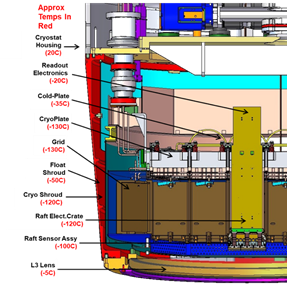
\includegraphics[width=2.18038in]{refrig/media/media/image2.png}

\textbf{Figure 1.3.1} Cross section of the cryostat with its principal thermal regions and typical design temperatures during operation (in red).

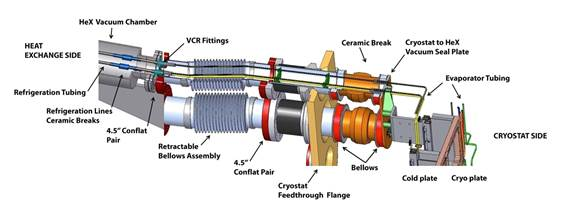
\includegraphics[width=5.98611in]{refrig/media/media/image1.jpg}

\textbf{Figure 1.3.2} Detailed routing of the refrigeration system at the interface between the cryostat and the heat exchanger vacuum system.

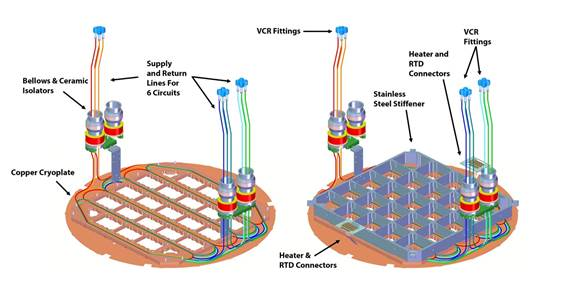
\includegraphics[width=6in]{refrig/media/media/image3.jpg}

\textbf{Figure 1.3.3} Cryoplate (a) Routing of six refrigerant circuits in the copper cryoplate (b) with stainless steel stiffening frame attached.

\textbf{Architecture of the Cryogenic Systems}

\begin{quote}
The physical layout of each cryo system is shown schematically in Figure 1.4.1.1 With the exception of the transfer line lengths, a largely identical system supports the camera in the clean room Maintenance Facility at the Vera C. Rubin Observatory.

All of the ground-based components reside in two temperature-controlled housings {[}``cryo cabinets''{]} attached to the underside of the Telescope Mount Assembly (TMA). The transfer lines to and from the camera (a liquid supply, a vapor supply, and a suction-return for each circuit) originate and return to these cabinets. They are a mix of orbitally welded - electropolished 316-L stainless steel tubing and flexible refrigerant lines which are insulated wherever possible. The counterflow HeX systems reside in a separate vacuum insulated housing within the camera's Utility Trunk, just behind the cryostat
\end{quote}
